\documentclass[10pt]{beamer}
\usetheme{jambro}
\graphicspath{{./graphics/}}


% Authors/institutes/date/etc
%--------------------------------
\title[]{Jambro Beamer Template}
\author[]{Ambrogio Cesa-Bianchi}
\date{\today}

\begin{document}

%=============================================================

\begin{frame}[plain]
	\titlepage{
		\begin{center}
			\begin{minipage}{0.8\textwidth}
				\centering
				\color{title!80}{\scriptsize *The Usual Disclaimer Applies}
			\end{minipage}
	\end{center}}
\end{frame}

%=============================================================
\section{Introduction}
\begin{frame}
	{Intro}
	\begin{itemize}
		\item After the usual \texttt{\textbackslash documentclass\{beamer\}} load the theme with \texttt{\textbackslash usetheme\{jambro\}}\bigskip
		\item The file \texttt{beamerthemejambro.sty} has to be in the same folder of your beamer presentation
	\end{itemize}
\end{frame}

%=============================================================

\begin{frame}
	{Intro}
	\begin{itemize}
		\item The theme comes with a few options to be specified in the \texttt{\textbackslash documentclass[option here]\{beamer\}} command \medskip
		\begin{itemize}
			\item \texttt{light}: uses Fira light as a default font\medskip
			\item \texttt{roboto}: changes the default font to Roboto\medskip
			\item \texttt{cabin}: changes the default font to Cabin\medskip
			\item \texttt{night}: switches to night mode colors \medskip
			\item \texttt{red}: switches the main color of the theme from blue to red (this option is overrun by \texttt{night})\medskip
			\item \texttt{3to2}: switches the aspect ratio from 16:9 to 3:2
		\end{itemize}
	\end{itemize}
\end{frame}

%=============================================================

\section{Tables \& Figures}
\begin{frame}
	\begin{eqnarray*}
		&\text{{\Huge \textbf{Tables \& Figures}}}\\
	\end{eqnarray*}
\end{frame}

%=============================================================

\begin{frame}
	{Tables}
	\begin{itemize}
		\item This is a table using \texttt{minipage} and \texttt{tabularx} commands
	\end{itemize}
	\begin{table}[th]
		\centering%
		\begin{minipage}[b]{.5\textwidth}
			\vspace{.2cm}\tablesize
			\begin{tabularx}{\textwidth}{lY}
				\toprule
				Dep. Variable: spread ($\Delta cs_{ij}$) 	& (1)\\
				\midrule
				& {Baseline Specification} \\
				\midrule
				\rowcolor{gray!10} Coeff. ($\beta_1$) 		&  21.15*** \\
				&   (7.35) \\
				\midrule
				\rowcolor{gray!10} Double clustering 		& Yes \\
				Time-sector FE 												& No \\
				\rowcolor{gray!10} R-squared 					& 0.034 \\
				Observations 												& 285,794 \\\bottomrule
			\end{tabularx}\vspace{.2cm}\newline
			\tiny{{\scshape Note.} Standard errors (reported in parentheses) are clustered two-way, at the firm level and time level. The asterisks denote statistical significance (*** for $p<0.01$, ** for $p<0.05$, * for $p<0.1$).\newline}%
			\label{tab:label}%
		\end{minipage}
	\end{table}
\end{frame}

%=============================================================

\begin{frame}
	{Tables}
	\begin{itemize}
		\item Control opacity of columns with \texttt{S} identifier within \texttt{tabularx} command 
	\end{itemize}
	\begin{table}[th]
		\centering%
		\begin{minipage}[b]{.5\textwidth}
			\vspace{.2cm}\tablesize
			\begin{tabularx}{\textwidth}{lS}
				\toprule
				Dep. Variable: spread ($\Delta cs_{ij}$) 	& (1)\\
				\midrule
				& {Baseline Specification} \\
				\midrule
				\rowcolor{gray!10} Coeff. ($\beta_1$) 		&  21.15*** \\
				&   (7.35) \\
				\midrule
				\rowcolor{gray!10} Double clustering 		& Yes \\
				Time-sector FE 												& No \\
				\rowcolor{gray!10} R-squared 					& 0.034 \\
				Observations 												& 285,794 \\\bottomrule
			\end{tabularx}\vspace{.2cm}\newline
			\tiny{{\scshape Note.} Standard errors (reported in parentheses) are clustered two-way, at the firm level and time level. The asterisks denote statistical significance (*** for $p<0.01$, ** for $p<0.05$, * for $p<0.1$).\newline}%
			\label{tab:label}%
		\end{minipage}
	\end{table}
\end{frame}

%=============================================================

\begin{frame}
	{Tables}
	\begin{itemize}
		\item Control the width of the table with \texttt{minipage} command \medskip
		\item The text in the columns from 2 onward is automatically place on multiple lines
	\end{itemize}
	\begin{table}[th]
		\centering%
		\begin{minipage}[b]{.4\textwidth}
			\vspace{.2cm}\tablesize
			\begin{tabularx}{\textwidth}{lY}
				\toprule
				Dep. Variable: spread ($\Delta cs_{ij}$) 	& (1)\\
				\midrule
				& {Baseline Specification} \\
				\midrule
				\rowcolor{gray!10} Coeff. ($\beta_1$) 		&  21.15*** \\
				&   (7.35) \\
				\midrule
				\rowcolor{gray!10} Double clustering 		& Yes \\
				Time-sector FE 												& No \\
				\rowcolor{gray!10} R-squared 					& 0.034 \\
				Observations 												& 285,794 \\\bottomrule
			\end{tabularx}\vspace{.2cm}\newline
			\tiny{{\scshape Note.} Standard errors (reported in parentheses) are clustered two-way, at the firm level and time level. The asterisks denote statistical significance (*** for $p<0.01$, ** for $p<0.05$, * for $p<0.1$).\newline}%
			\label{tab:label}%
		\end{minipage}
	\end{table}
\end{frame}

%=============================================================

\begin{frame}
	{Figures}
	\begin{itemize}
		\item This is a figure
	\end{itemize}
	\begin{center}
		\begin{minipage}[b]{.6\textwidth}
			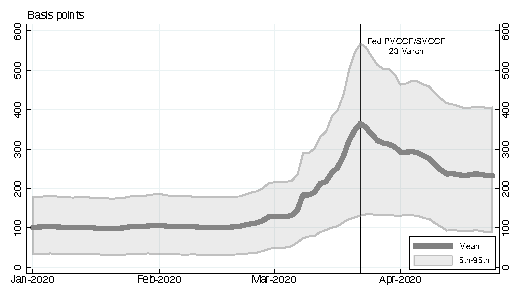
\includegraphics[width=\textwidth]{Figure.pdf}\\
			\tiny{{\scshape Note}. \ Global average of investment grade corporate bond spreads (option-adjusted) weighted by bonds face value, together with 5th and 95th percentile of the full distribution. Source: ICE BoA ML.}
		\end{minipage}
	\end{center}
\end{frame}


%=============================================================

\section{Arrows \& Handwriting}
\begin{frame}
	\begin{eqnarray*}
		&\text{{\Huge \textbf{Arrows \& Handwriting}}}\\
	\end{eqnarray*}
\end{frame}

%=============================================================

\begin{frame}[t]
	{Arrows and handwritten notes}\bigskip
	\begin{itemize}
		\item The theme embeds a way to introduce handwritten notes using arrows \bigskip\medskip
		\item Imagine you want to clarify something about \tikz[tstyle]{\node[nstyle](node1){$x$}} \bigskip\medskip\pause
		\item The theme allows to add arrows and handwritten notes using Tikz in combination with the \texttt{\textbackslash hand} command \medskip
		\begin{itemize}
			\item Arrows can start from different cardinal points 
			\begin{tikzpicture}[tpstyle]
				\draw[arrow,->] ([yshift=2pt]node1.north east) to[bend left] +(0.7,+0.3) node[anchor=west] {\small{\hand A comment from the north}};
				\draw[arrow,->] ([yshift=-2pt]node1.south) to[bend right] +(1.6,-0.2) node[anchor=west] {\small{\hand A comment from the south}};
			\end{tikzpicture}	
		\end{itemize}
	\end{itemize}
\end{frame}

%=============================================================

\begin{frame}[t]
	{Arrows and handwritten notes}\bigskip
	\begin{itemize}
		\item The theme embeds a way to introduce handwritten notes using arrows \bigskip\medskip
		\item Imagine you want to clarify something about \tikz[tstyle]{\node[nstyle](node1){$x$}} \bigskip\medskip
		\item The theme allows to add arrows and handwritten notes using Tikz in combination with the \texttt{\textbackslash hand} command \medskip
		\begin{itemize}
			\item Arrows can start from different cardinal points... \medskip
			\item ...have different colors and opacity... \medskip
			\begin{tikzpicture}[tpstyle]
				\draw[arrow,->,brick,opacity=0.5] ([yshift=2pt]node1.north east) to[bend left] +(0.7,+0.3) node[brick,anchor=west,opacity=0.5] {\small{\hand A comment from the north}};
				\draw[arrow,->,brick] ([yshift=-2pt]node1.south) to[bend right] +(1.6,-0.2) node[brick,anchor=west] {\small{\hand A comment from the south}};
			\end{tikzpicture}	
		\end{itemize}
	\end{itemize}
\end{frame}


%=============================================================

\begin{frame}[t]
	{Arrows and handwritten notes}\bigskip
	\begin{itemize}
		\item The theme embeds a way to introduce handwritten notes using arrows \bigskip\medskip
		\item Imagine you want to clarify something about \tikz[tstyle]{\node[nstyle](node1){$x$}} \bigskip\medskip
		\item The theme allows to add arrows and handwritten notes using Tikz in combination with the \texttt{\textbackslash hand} command \medskip
		\begin{itemize}
			\item Arrows can start from different cardinal points... \medskip
			\item ...have different colors and opacity... \medskip
			\item ...have wiggles....
			\begin{tikzpicture}[tpstyle]
				\draw[arrow,->,brick,opacity=0.5] ([yshift=2pt]node1.north east) to[bend left] +(0.7,+0.3) node[brick,anchor=west,opacity=0.5] {\small{\hand A comment from the north}};
				\draw[snake,->,brick] ([yshift=-2pt]node1.south) to[bend right] +(1.6,-0.2) node[brick,anchor=west] {\small{\hand A comment from the south}};
			\end{tikzpicture}	
		\end{itemize}
	\end{itemize}
\end{frame}

%=============================================================

\begin{frame}[t]
	{Arrows and handwritten notes}\bigskip
	\begin{itemize}
		\item The theme embeds a way to introduce handwritten notes using arrows \bigskip\medskip
		\item Imagine you want to clarify something about \tikz[tstyle]{\node[nstyle](node1){$x$}} \bigskip\medskip
		\item The theme allows to add arrows and handwritten notes using Tikz in combination with the \texttt{\textbackslash hand} command \medskip
		\begin{itemize}
			\item Arrows can start from different cardinal points... \medskip
			\item ...have different colors and opacity... \medskip
			\item ...have wiggles... \medskip
			\item ...be bidirectional or adirectional
			\begin{tikzpicture}[tpstyle]
				\draw[arrow,brick,opacity=0.5] ([yshift=2pt]node1.north east) to[bend left] +(0.7,+0.3) node[brick,anchor=west,opacity=0.5] {\small{\hand A comment from the north}};
				\draw[snake,<->,brick] ([yshift=-2pt]node1.south) to[bend right] +(1.6,-0.2) node[brick,anchor=west] {\small{\hand A comment from the south}};
			\end{tikzpicture}	
		\end{itemize}
	\end{itemize}
\end{frame}

%=============================================================

\begin{frame}[t]
	{Handwritten notes to figures}
	\begin{itemize}
		\item Add notes to figures using the \texttt{tikzpicture} environment
	\end{itemize}
	\begin{center}
		\begin{minipage}[b]{.6\textwidth}
			\begin{tikzpicture}
				\node[inner sep=0] (image) at (0,0) {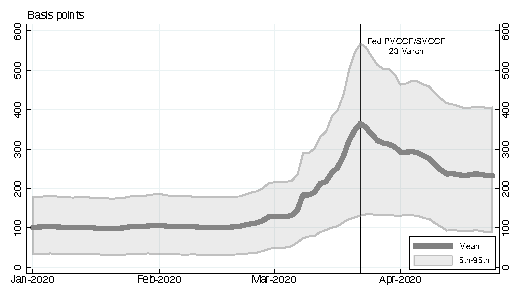
\includegraphics[width=\textwidth]{Figure.pdf}};
				\draw[arrow,->,opacity=1] (1,0.4) to[bend right] +(-1,+0.9) node[anchor=east,opacity=1] {\normalsize{\hand - One comment}};
				\draw[arrow,->,opacity=1,brick] (0.8,0.4) to[bend right] +(-0.8,-0.6)  node[anchor=east,opacity=1,brick] {\normalsize{\hand - Another comment}};
			\end{tikzpicture}
			\tiny{{\scshape Note}. \ Global average of investment grade corporate bond spreads (option-adjusted) weighted by bonds face value, together with 5th and 95th percentile of the full distribution. Source: ICE BoA ML.} 
		\end{minipage}
	\end{center}
\end{frame}	

%=============================================================

\begin{frame}[t]
	{Handwritten notes to figures}
	\begin{itemize}
		\item Add shaded areas on top of figures with the \texttt{tikzpicture} environment
	\end{itemize}
	\begin{center}
		\begin{minipage}[b]{.6\textwidth}
			\begin{tikzpicture}
				\node[inner sep=0] (image) at (0,0) {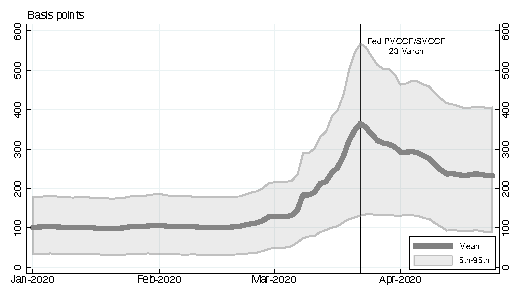
\includegraphics[width=\textwidth]{Figure.pdf}};
				\draw[arrow,->,opacity=1] (1,0.4) to[bend right] +(-1,+0.9) node[anchor=east,opacity=1] {\normalsize{\hand - One comment}};
				\draw[arrow,->,opacity=1,brick] (0.8,0.4) to[bend right] +(-0.8,-0.6)  node[anchor=east,opacity=1,brick] {\normalsize{\hand - Another comment}};
				\node[rectangle,fill=gold,opacity=0.2,rounded corners=.1cm,minimum width=2cm,minimum height = 5cm] at (0.9,0) {};
			\end{tikzpicture}
			\tiny{{\scshape Note}. \ Global average of investment grade corporate bond spreads (option-adjusted) weighted by bonds face value, together with 5th and 95th percentile of the full distribution. Source: ICE BoA ML.} 
		\end{minipage}
	\end{center}
\end{frame}	

%=============================================================

\section{Highlighting}
\begin{frame}
	\begin{eqnarray*}
		&\text{{\Huge \textbf{Highlighting}}}\\
	\end{eqnarray*}
\end{frame}

%=============================================================

\begin{frame}
	{Underlying}
	\begin{itemize}
		\item Highlight text with the \hlight{\texttt{\textbackslash hlight\{\}}} command \bigskip
		\item Or highlight text with a `pencil underline' effect using Tikz \medskip
		\begin{itemize}
			\item \tikz[tstyle]{\node[nstyle](node2){Highlight text with a pencil}}
			\begin{tikzpicture}[tpstyle]
				\draw[pencil] ([yshift=-2pt]node2.south west) to ([yshift=-2pt]node2.south east);			
			\end{tikzpicture}  \bigskip \pause
			\item \tikz[tstyle]{\node[nstyle](node2){Highlight text with a thicker pencil}}
			\begin{tikzpicture}[tpstyle]
				\draw[pencil,very thick] ([yshift=-2pt]node2.south west) to ([yshift=-2pt]node2.south east);			
			\end{tikzpicture}  \bigskip \pause
			\item \tikz[tstyle]{\node[nstyle](node2){Highlight text with a different color thicker pencil}}
			\begin{tikzpicture}[tpstyle]
				\draw[pencil,very thick,brick] ([yshift=-2pt]node2.south west) to ([yshift=-2pt]node2.south east);			
			\end{tikzpicture} 
		\end{itemize}
	\end{itemize}
\end{frame}

%=============================================================

\begin{frame}
	{Boxing text or variables in equations}
	\begin{itemize}
		\item Highlight text with a \tikz[tstyle]{\node[nstyle](node0){pencil box}} effect using Tikz \bigskip\bigskip
		\begin{tikzpicture}[tpstyle]
			\node[pencil,draw, minimum height=0.7cm, minimum width=1.7cm] (box0) at (node0) {};
		\end{tikzpicture}\pause
		\item Or highlight objects in equations with a thicker box \medskip
		\begin{equation*}
			y_{t} = \alpha + \tikz[tstyle]{\node[nstyle](node1){$\beta x_t$}} + u_{t}
		\end{equation*}
		\smallskip
		\begin{tikzpicture}[tpstyle]
			\node[pencil,very thick,draw, minimum height=0.8cm, minimum width=0.8cm] (box1) at (node1) {};
		\end{tikzpicture}\pause
		\item Add arrows and comments using \texttt{\textbackslash draw[arrow]}
		\begin{tikzpicture}[tpstyle]
			\draw[arrow,->] ([yshift=2pt]box1.north east) to[bend left] +(+0.7,0.5) node[anchor=west,opacity=1] {\hand A comment from north east};
		\end{tikzpicture}
	\end{itemize}
\end{frame}

%=============================================================

\begin{frame}
	{Boxing numbers in a table}
	\begin{table}[th]
		\centering%
		\begin{minipage}[b]{.6\textwidth}
			\vspace{.2cm}\tablesize
			\begin{tabularx}{\textwidth}{lY}
				\toprule
				Dep. Variable: spread ($\Delta cs_{ij}$) 	& (1)\\
				\midrule
				& {Baseline Specification} \\
				\midrule
				\rowcolor{gray!10} Coeff. ($\beta_1$) 		&  {\tikz[tstyle]{\node[nstyle](node1){21.15***}}} \\
				&   (7.35) \\
				\midrule
				\rowcolor{gray!10} Double clustering 		& Yes \\
				Time-sector FE 												& No \\
				\rowcolor{gray!10} R-squared 					& 0.034 \\
				Observations 												& 285,794 \\\bottomrule
			\end{tabularx}\vspace{.2cm}\newline
			\tiny{{\scshape Note.} Standard errors (reported in parentheses) are clustered two-way, at the firm level and time level. The asterisks denote statistical significance (*** for $p<0.01$, ** for $p<0.05$, * for $p<0.1$).\newline}%
			\label{tab:label}%
		\end{minipage}
	\end{table}
	\begin{tikzpicture}[tpstyle]
		\node[pencil,draw, minimum height=0.4cm, minimum width=1.1cm] (box1) at (node1) {};
	\end{tikzpicture}
\end{frame}

%=============================================================

\section{Sketches}
\begin{frame}
	\begin{eqnarray*}
		&\text{{\Huge \textbf{Sketches}}}\\
	\end{eqnarray*}
\end{frame}


%=============================================================

\begin{frame}{Sketch of a model}
	\begin{center}
		\begin{tikzpicture}
			% HOME
			%--------------
			% Home Banks
			\node[fill=title!70,text=white,rounded corners,inner sep=1ex,font=\bfseries,xshift=0cm,yshift=0cm] (Bank) {Home Banks};
			% Home Firm
			\node[fill=title!70,text=white,rounded corners,inner sep=1ex,font=\bfseries,xshift=+5.5cm,yshift=0cm] (Hfirm) {Home Non-financial Firms};
			% Home Households
			\node[fill=title!70,text=white,rounded corners,inner sep=1ex,font=\bfseries,xshift=-3.5cm,yshift=-3cm] (Hhh) {Home Households};
			% Arrows 
			\draw[arrow,black,->,very thick] ([xshift=0.2cm]Bank.east) to ([xshift=-0.2cm]Hfirm.west);
			\draw[snake,black,->,very thick] ([xshift=0.2cm]Hhh.east) to [bend right] ([yshift=-0.2cm]Bank.south);
			% Labels
			\draw[] (1.1cm,-1.6cm) node[anchor=north,opacity=1,] {\small \hand LC deposits};
			\draw[title!70] (1.1cm,-2cm) node[anchor=north,opacity=1,] {\small \hand \footnotesize{Agency friction}};
			\draw[] (2.1cm,.6cm) node[anchor=north,opacity=1,] {\small \hand Securities};
			% US
			%--------------
			% US Household
			\node[fill=title!70,text=white,rounded corners,inner sep=1ex,font=\bfseries,xshift=-3.5cm,yshift=3cm] (Fhh) {US Household};
			% Arrows 
			\draw[snake,black,->,very thick] ([xshift=0.2cm]Fhh.east) to [bend left] ([yshift=0.2cm]Bank.north);
			% Labels
			\draw[] (-2.3cm,2.4cm) node[anchor=north,opacity=1,] {\small \hand USD deposits};
			\draw[title!70] (-2.3cm,2cm) node[anchor=north,opacity=1,] {\hand \footnotesize{More severe}};
			\draw[title!70] (-2.3cm,1.7cm) node[anchor=north,opacity=1,] {\hand \footnotesize{Agency friction}};
			% SWAP LINES
			%--------------
			% Fed
			\node[fill=title!70,text=white,rounded corners,inner sep=1ex,font=\bfseries,xshift=-5.5cm,yshift=1.5cm] (Fed) {Fed};
			% Home CB
			\node[fill=title!70,text=white,rounded corners,inner sep=1ex,font=\bfseries,xshift=-4.5cm,yshift=-1cm] (CB) {Home Central Bank};
			% Arrows 
			\draw[arrow,black,<->,very thick] ([xshift=0cm]Fed.south west) to [bend right] ([xshift=-0cm]CB.north west);
			\draw[arrow,black,->,very thick] ([xshift=0.2cm]CB.east) to [bend right] ([xshift=-0cm]Bank.south west);
			% Labels
			\draw[] (-5.3cm,0.5cm) node[anchor=north,opacity=1] {\small \hand Swap line};
			\draw[] (-2cm,0.1cm) node[anchor=north,opacity=1] {\small \hand USD};
			\draw[] (-2cm,-0.2cm) node[anchor=north,opacity=1] {\small \hand funds};
		\end{tikzpicture}
	\end{center}
\end{frame}

%=============================================================

\begin{frame}{Sketch of demand and supply}
	\begin{center}
		\begin{tikzpicture}[scale=1.9, important line/.style={thick}, dashed line/.style={dashed, thin}, every node/.style={color=black}, dot/.style={circle,fill=black,minimum size=5.5pt,inner sep=0pt,outer sep=-1pt}]
			% Axes
			\draw[thick, ->, >=stealth', line join=miter,<->](3,0) 
			node(xline)[below,xshift=-2.5cm, yshift=-.1cm] {\small{\hand Capital $(K)$}} -| (0,2.5) 
			node(yline)[above,rotate=90,xshift=-2.5cm, yshift=1cm] {\small{\hand Credit Spread $\left(R^B/R\right)$}};
			% Demand
			\draw[scale=0.5,domain=1.7:2.9,smooth,variable=\x,thick,gray,opacity=0.6]  plot ({\x}, {3-4*ln(\x-1)}) node[right, opacity=1] {\footnotesize{\hand Demand $(K^D_{j,\ell})$}};
			% Supply LOW
			\draw[scale=0.5,domain=0:1.2,smooth,variable=\x,thick,red] plot ({\x},  {1});
			\node[label=left: $1$] at (0,0.5) (int1) {};	
			\draw[scale=0.5,domain=1.2:2.35,smooth,variable=\x,thick,red] plot ({\x},  {1+2*(\x-1.2)^2}) node[right] {\footnotesize{\hand Supply $(K^S_{j,\ell})$}};
			% Equilibria
			\node[circle,draw=black, fill=red,inner sep=1.25pt] at (1.05,1.3) (int1) {};
			\node[label=\footnotesize  $\mathcal{A}_\ell$] at (0.89,1.12) (int1) {};
		\end{tikzpicture}
		\begin{tikzpicture}[scale=1.9, important line/.style={thick}, dashed line/.style={dashed, thin}, every node/.style={color=black}, dot/.style={circle,fill=black,minimum size=5.5pt,inner sep=0pt,outer sep=-1pt}]
			% Axes
			\draw[thick, ->, >=stealth', line join=miter,<->](3,0) 
			node(xline)[below,xshift=-2.5cm, yshift=-.1cm] {\small{\hand Capital $(K)$}} -| (0,2.5);
			% Demand
			\draw[scale=0.5,domain=1.7:2.9,smooth,variable=\x,thick,gray,opacity=0.6]  plot ({\x}, {3-4*ln(\x-1)}) node[right, opacity=1] {\footnotesize{\hand Demand $(K^D_{j,h})$}};
			% Supply HIGH 
			\draw[scale=0.5,domain=0:2,smooth,variable=\x,thick,main] plot ({\x},  {1});
			\node[label=left: $1$] at (0,0.5) (int1) {};	
			\draw[scale=0.5,domain=2:3.5,smooth,variable=\x,thick,main] plot  ({\x}, {1+0.6*(\x-2)^2}) node[right] {\footnotesize{\hand Supply $(K^S_{j,h})$}};
			% Equilibria
			\node[circle,draw=black, fill=main,inner sep=1.25pt] at (1.29,0.6) (int1) {};
			\node[label=\footnotesize  $\mathcal{A}_h$] at (1.45,0.35) (int1) {};
		\end{tikzpicture}
	\end{center}
\end{frame}

%=============================================================

\begin{frame}
	{Bubbles}
	\begin{itemize}
		\item The theme allows to create bubbles with the \texttt{\textbackslash NB} command in combination with the \texttt{minipage} environment \bigskip
	\end{itemize}
	\begin{center}
		\begin{minipage}{.4\textwidth}
			\NB{This is a small bubble}
		\end{minipage}
	\end{center}
	\begin{center}
		\begin{minipage}{.6\textwidth}
			\NB{This is a large bubble.\\ With two lines}
		\end{minipage}
	\end{center}
	\begin{center}
		\begin{minipage}{.8\textwidth}
			\NB{This is a larger bubble with bullets:
				\begin{itemize}
					\item Uno
					\item Dos
					\item Tres 
			\end{itemize}}
		\end{minipage}
	\end{center}
\end{frame}


%=============================================================

\end{document}


